\newpage
\appendix

\section*{Appendix}

\subsection*{DC Charger Network Details}

Network characteristics for DC charging networks in California are shown in Figure \ref{fig:ris_top_networks} and in Table \ref{tab:summary_statistics_afdc}. Data pulled from \gls{afdc} in May 2024.

\begin{figure}[H]
	\centering
	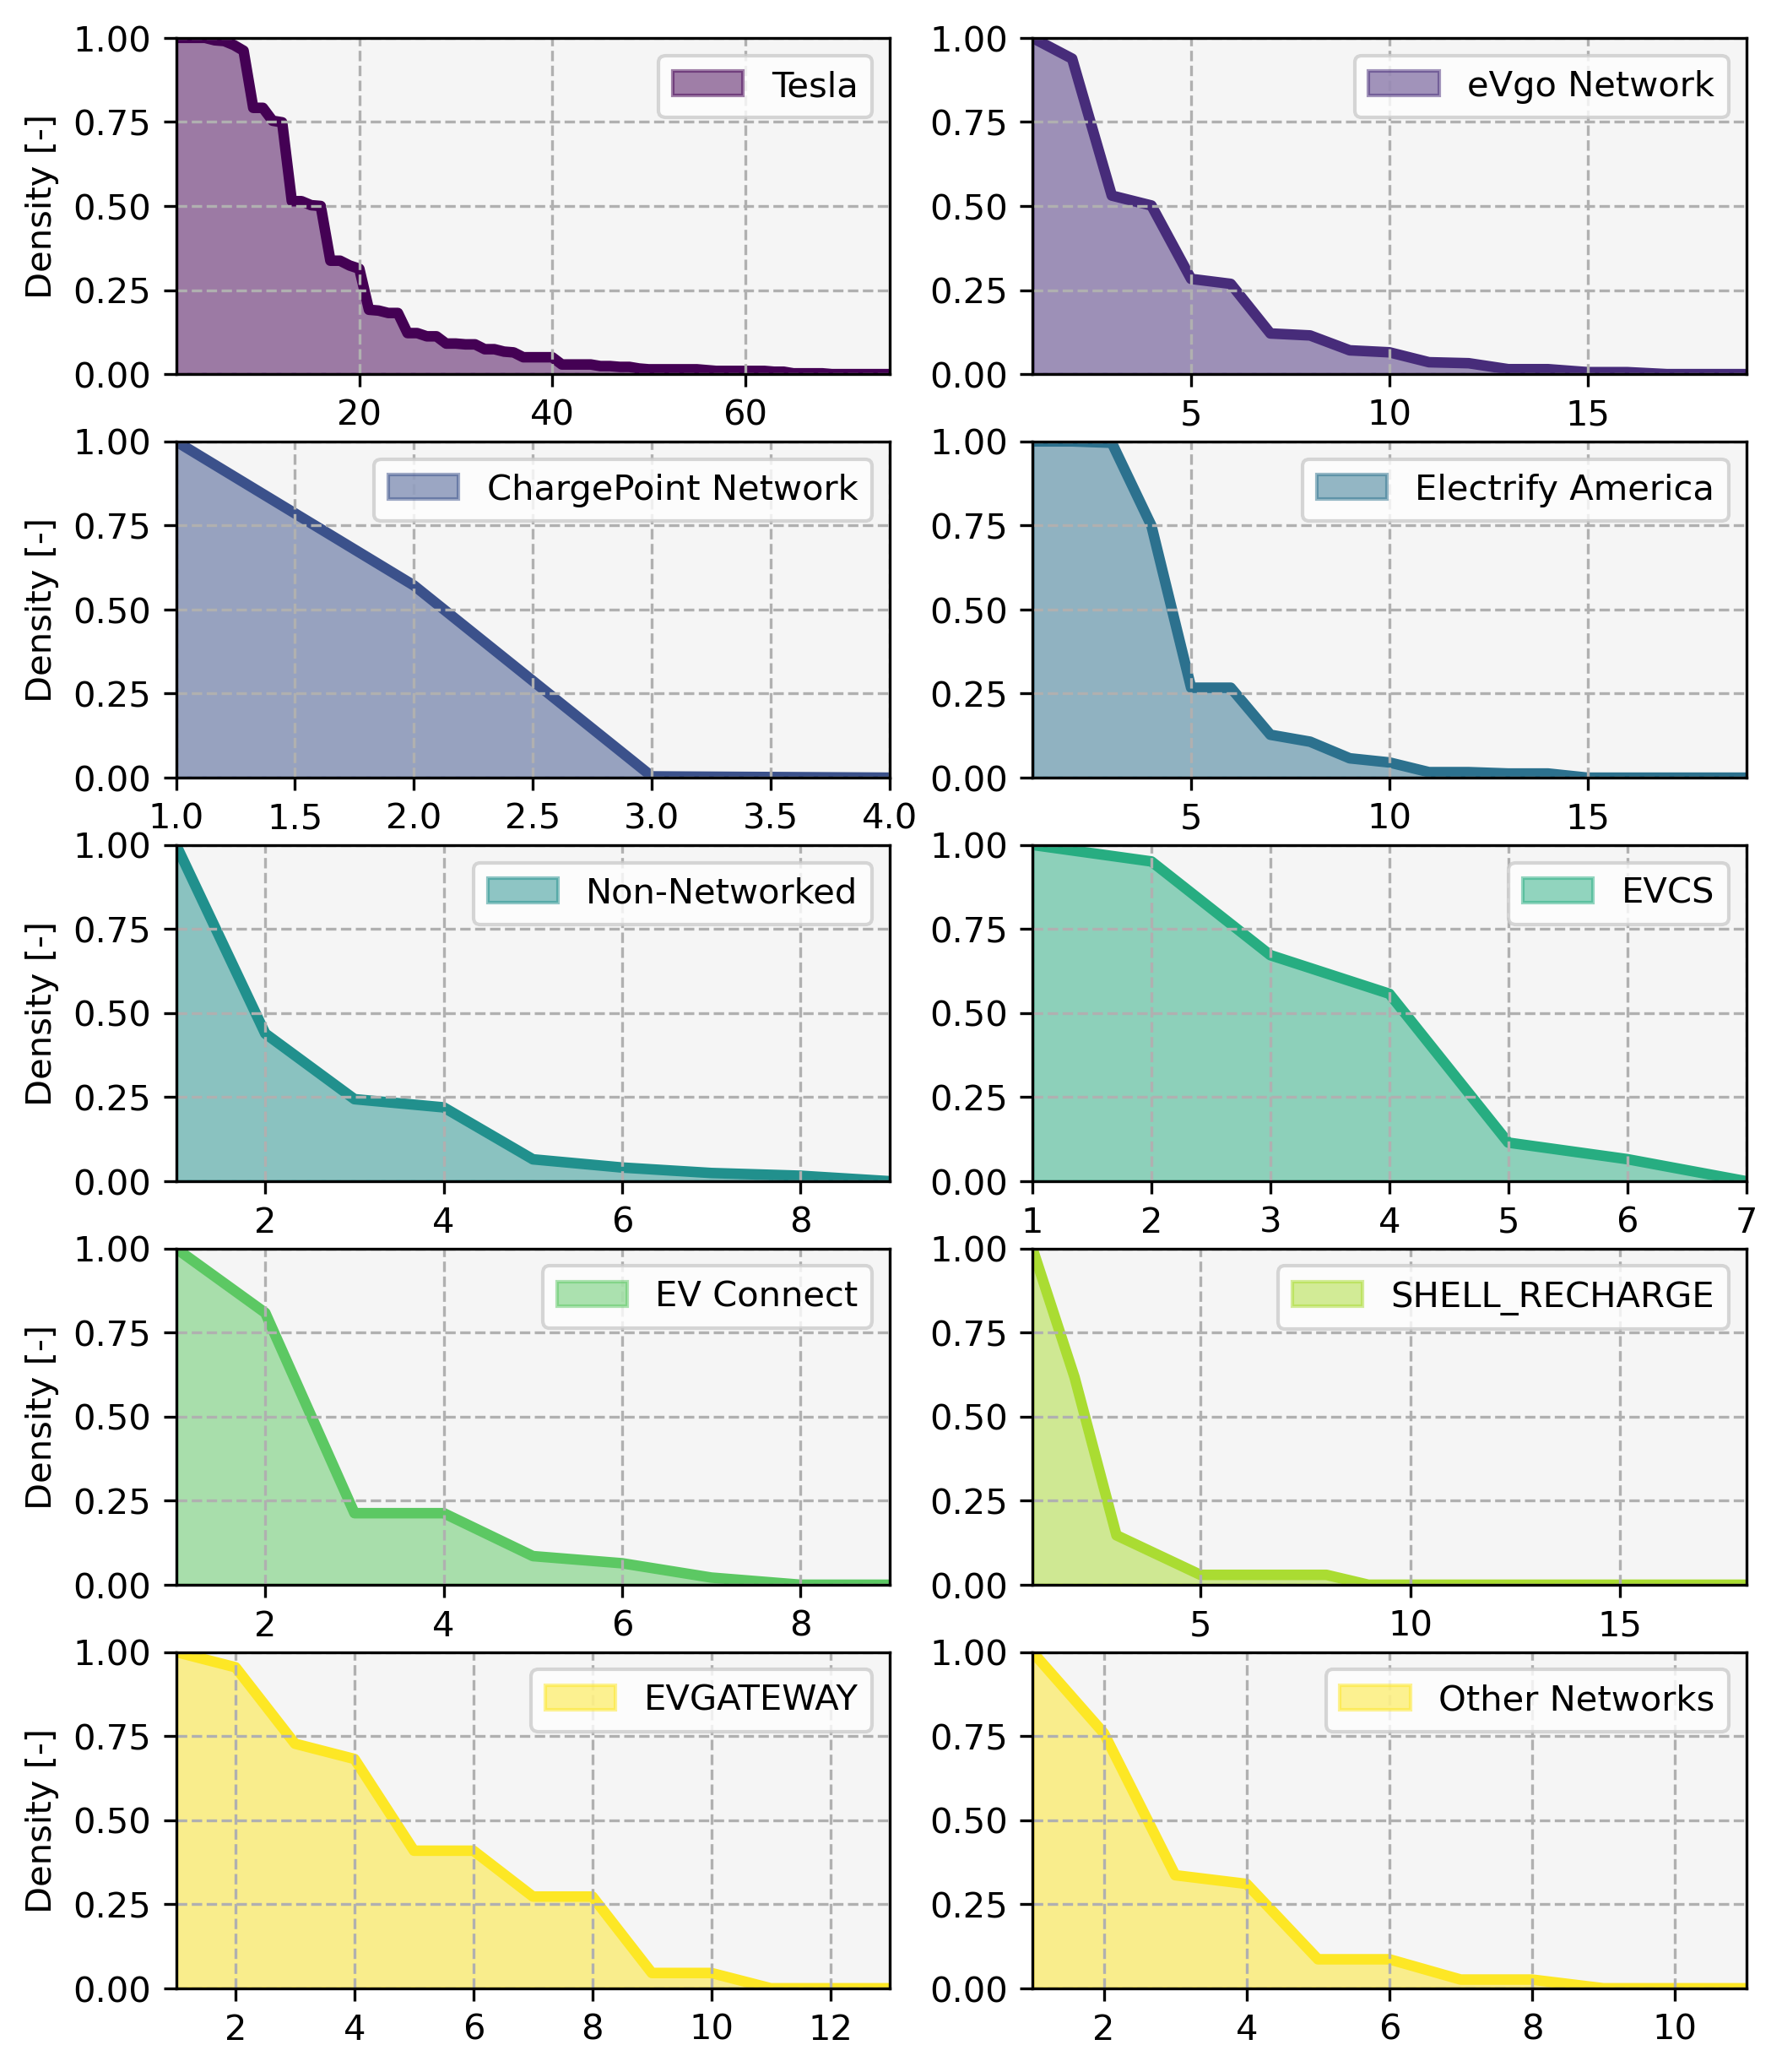
\includegraphics[width = \linewidth]{figs/California_RIS_SF_All.png}
	\caption{In-station redundancy for DC Charging networks in California}
	\label{fig:ris_top_networks}
\end{figure}

\begin{table}[H]
	\centering
	\caption{Summary statistics for California DC charging networks from \gls{afdc}}
	\label{tab:summary_statistics_afdc}
	\begin{tabular}{|C{.46\linewidth}|C{.18\linewidth}|C{.18\linewidth}|C{.18\linewidth}|}
		\hline Network & Chargers & Stations & Chargers per Station \\
		\hline Non-Networked & 288 & 51 & 5.6 \\
		\hline Tesla & 2753 & 156 & 17.6 \\
		\hline Electrify America & 526 & 77 & 6.8 \\
		\hline EV Connect & 59 & 19 & 3.1 \\
		\hline ChargePoint Network & 186 & 79 & 2.4 \\
		\hline Volta & 2 & 2 & 1.0 \\
		\hline EVCS & 41 & 11 & 3.7 \\
		\hline SHELL_RECHARGE & 39 & 11 & 3.5 \\
		\hline EVGATEWAY & 21 & 5 & 4.2 \\
		\hline eVgo Network & 332 & 63 & 5.3 \\
		\hline BP_PULSE & 3 & 2 & 1.5 \\
		\hline POWERFLEX & 12 & 3 & 4.0 \\
		\hline FLO & 1 & 1 & 1.0 \\
		\hline EVRANGE & 11 & 3 & 3.7 \\
		\hline RIVIAN_ADVENTURE & 14 & 7 & 2.0 \\
		\hline CIRCLE_K & 16 & 3 & 5.3 \\
		\hline CHARGENET & 7 & 1 & 7.0 \\
		\hline Blink Network & 2 & 2 & 1.0 \\
		\hline NOODOE & 2 & 1 & 2.0 \\
		\hline LOOP & 6 & 2 & 3.0 \\
		\hline 7CHARGE & 4 & 1 & 4.0 \\
		\hline
	\end{tabular}
\end{table}

Network characteristics for DC charging networks in California, conunting only corridor chargers, are shown in Figure \ref{fig:ris_top_networks} and in Table \ref{tab:summary_statistics_afdc}. Data pulled from \gls{afdc} in May 2024.

\begin{figure}[H]
	\centering
	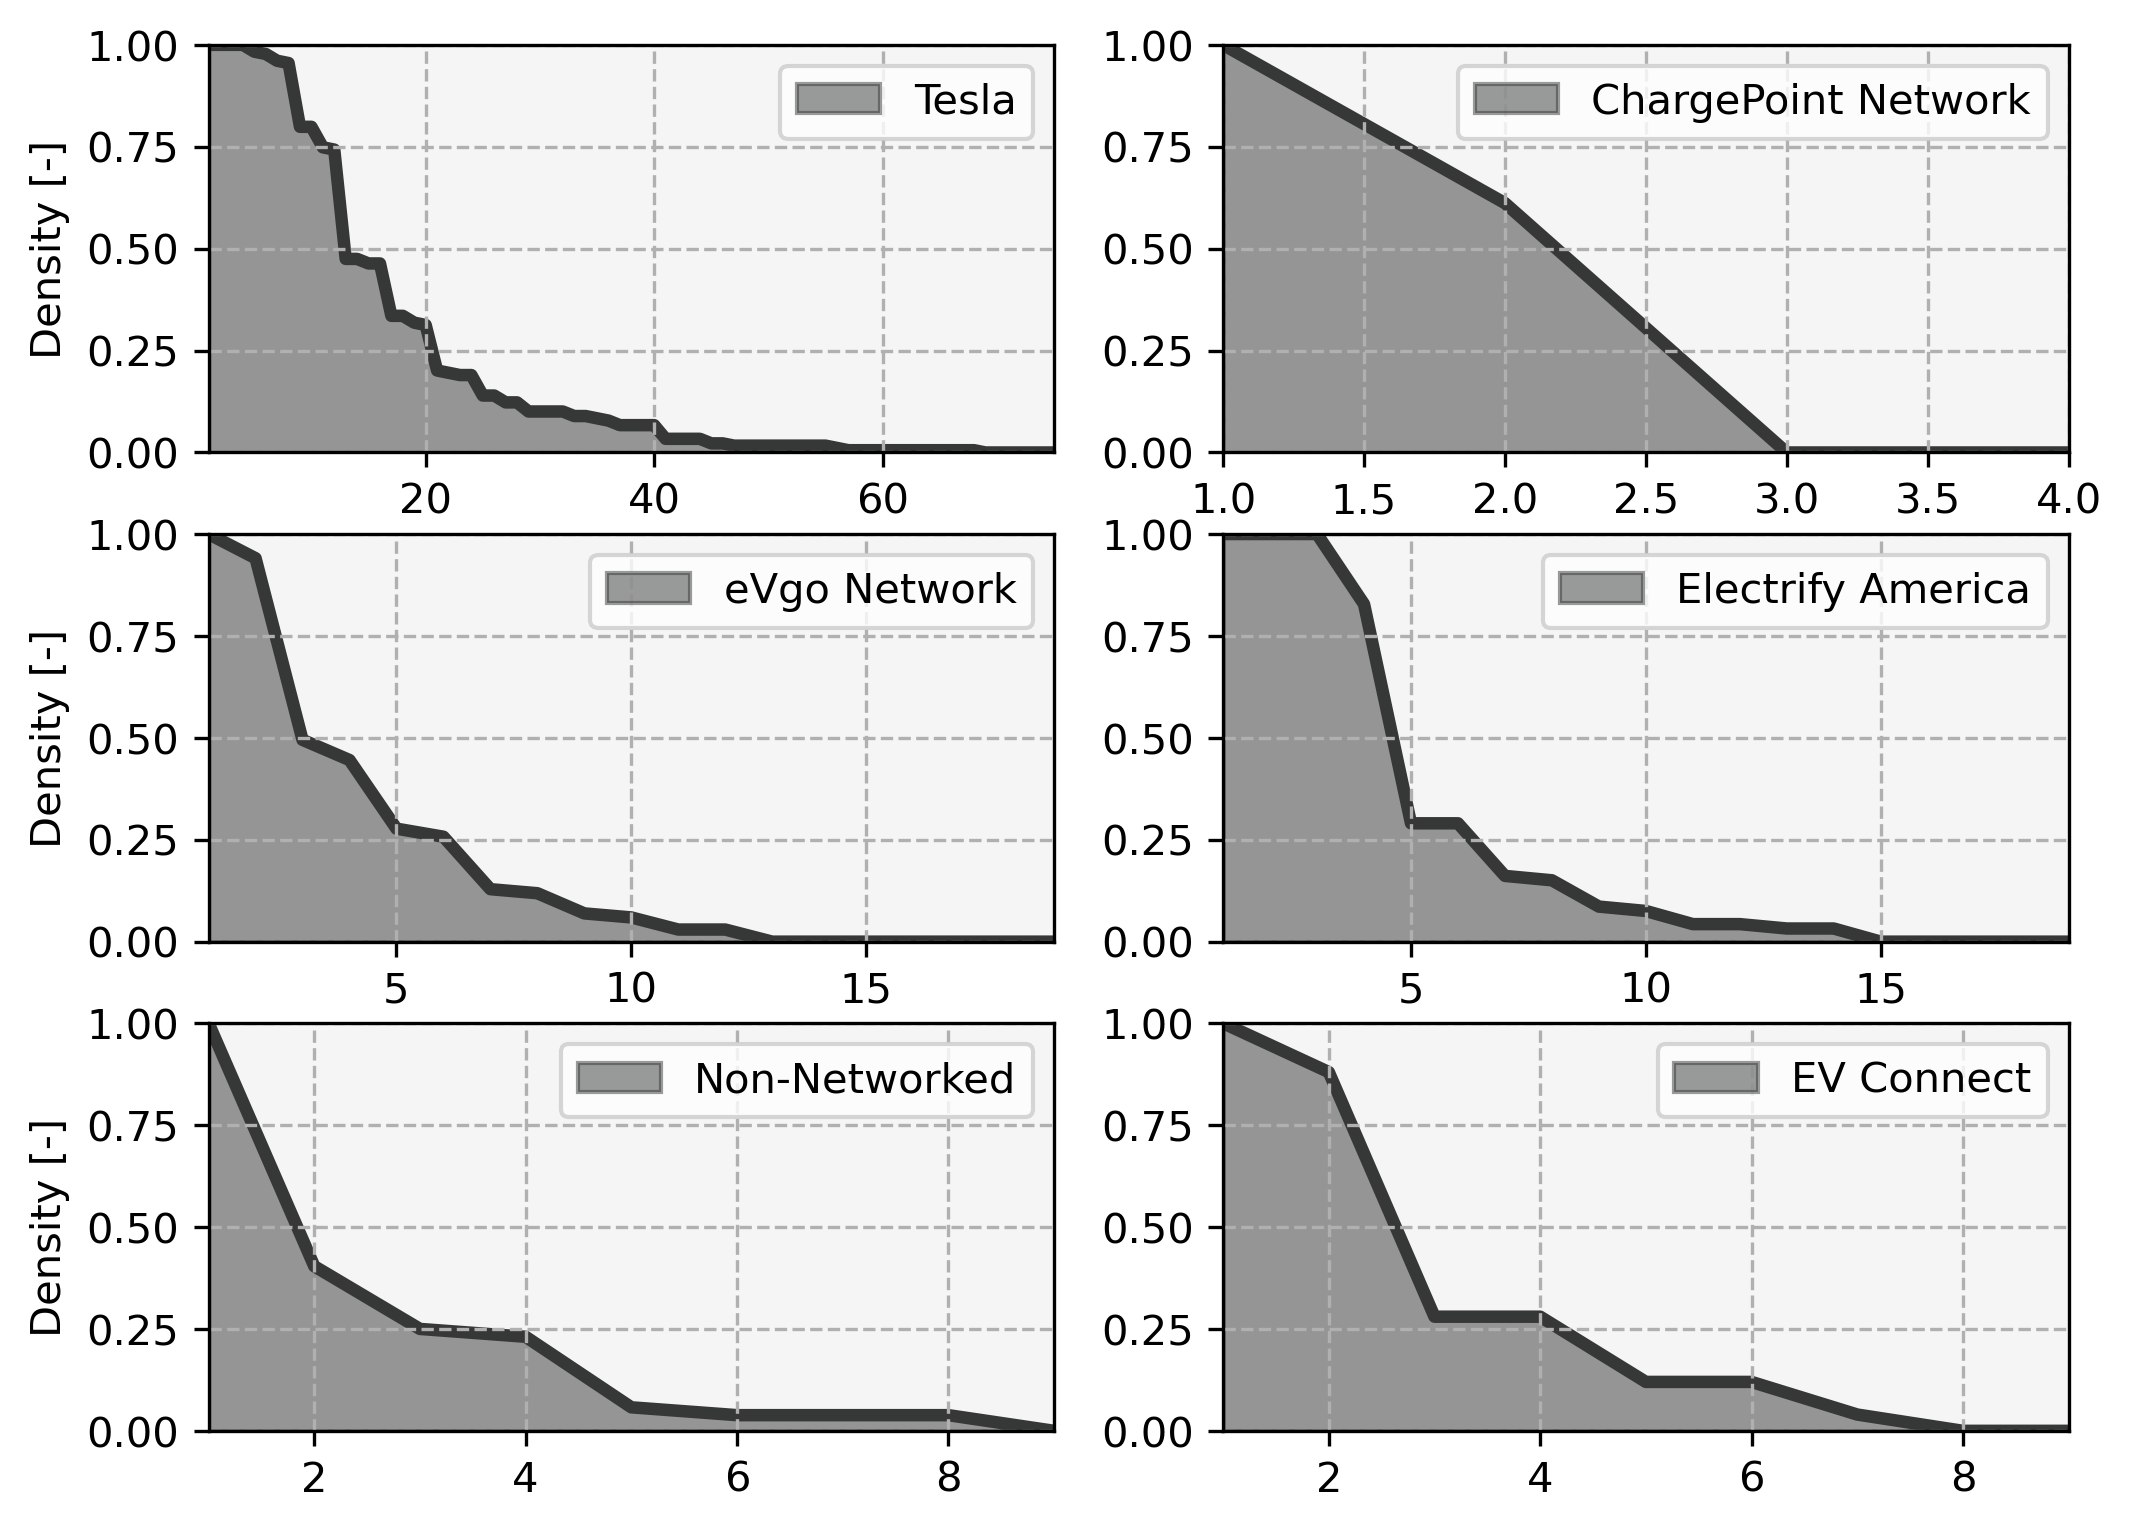
\includegraphics[width = \linewidth]{figs/California_RIS_SF_Corridor.png}
	\caption{In-station redundancy for DC Charging networks in California}
	\label{fig:ris_top_networks_corridor}
\end{figure}

\begin{table}[H]
	\centering
	\caption{Summary statistics for California DC charging networks from \gls{afdc} (corridor stations)}
	\label{tab:summary_statistics_afdc_corridor}
	\begin{tabular}{|C{.46\linewidth}|C{.18\linewidth}|C{.18\linewidth}|C{.18\linewidth}|}
		\hline Network & Chargers & Stations & Chargers per Station \\
		\hline Non-Networked & 274 & 50 & 5.5 \\
		\hline Tesla & 2745 & 155 & 17.7 \\
		\hline Electrify America & 518 & 76 & 6.8 \\
		\hline EV Connect & 58 & 18 & 3.2 \\
		\hline ChargePoint Network & 184 & 78 & 2.4 \\
		\hline Volta & 1 & 1 & 1.0 \\
		\hline EVCS & 35 & 10 & 3.5 \\
		\hline SHELL_RECHARGE & 37 & 10 & 3.7 \\
		\hline EVGATEWAY & 19 & 4 & 4.8 \\
		\hline eVgo Network & 329 & 62 & 5.3 \\
		\hline BP_PULSE & 1 & 1 & 1.0 \\
		\hline POWERFLEX & 10 & 2 & 5.0 \\
		\hline EVRANGE & 5 & 2 & 2.5 \\
		\hline RIVIAN_ADVENTURE & 12 & 6 & 2.0 \\
		\hline CIRCLE_K & 12 & 2 & 6.0 \\
		\hline Blink Network & 1 & 1 & 1.0 \\
		\hline LOOP & 2 & 1 & 2.0 \\
		\hline
	\end{tabular}
\end{table}

\subsection*{Regression Details}

Details of linear regression on random experiment results are displayed in the following tables. Tables \ref{tab:regression_anova_c} and \ref{tab:regression_coefficients_c} concern the combined network, Tables \ref{tab:regression_anova_t} and \ref{tab:regression_coefficients_t} concern the Tela network, and Tables \ref{tab:regression_anova_nt} and \ref{tab:regression_coefficients_nt} concern the non-Tesla network.

\begin{table}[H]
	\centering
	\caption{Combined Network Linear Regression Analysis ANOVA}
	\label{tab:regression_anova_c}
	\begin{tabular}{|C{.25\linewidth}|C{.25\linewidth}|C{.25\linewidth}|C{.25\linewidth}|}
		\hline R & R-Squared & Adjusted R-Squared & Std. Error \\
		\hline 0.926 & 0.858 & 0.853 & 0.000 \\
		\hline
		\hline Category & Sum of Squares & DOF & Mean Squares \\
		\hline Model & 28.706 & 15 & 1.914 \\
		\hline Error & 4.754 & 484 & 0.010 \\
		\hline Total & 33.460 & 499 & 0.067 \\
		\hline  \multicolumn{2}{|c|}{$F$} &  \multicolumn{2}{c|}{$P(>F)$}  \\
		\hline  \multicolumn{2}{|c|}{194.848} &  \multicolumn{2}{c|}{0.000}  \\
		\hline
	\end{tabular}
\end{table}

\begin{table}[H]
	\centering
	\caption{Combined Network Linear Regression Analysis Coefficients}
	\label{tab:regression_coefficients_c}
	\begin{tabular}{|C{.5\linewidth}|C{.25\linewidth}|C{.25\linewidth}|}
		\hline Parameter & Coefficient & P-Value \\
		\hline {\small Intercept } & 7.121 & 0.000 \\
		\hline {\small power } & -1.009 & 0.000 \\
		\hline {\small capacity } & -1.031 & 0.000 \\
		\hline {\small reliability } & -0.227 & 0.040 \\
		\hline {\small capacity:power } & 0.984 & 0.000 \\
		\hline {\small capacity:reliability } & 0.422 & 0.036 \\
		\hline
	\end{tabular}
\end{table}

\begin{table}[H]
	\centering
	\caption{Tesla Network Linear Regression Analysis ANOVA}
	\label{tab:regression_anova_t}
	\begin{tabular}{|C{.25\linewidth}|C{.25\linewidth}|C{.25\linewidth}|C{.25\linewidth}|}
		\hline R & R-Squared & Adjusted R-Squared & Std. Error \\
		\hline 0.926 & 0.857 & 0.852 & 0.000 \\
		\hline
		\hline Category & Sum of Squares & DOF & Mean Squares \\
		\hline Model & 27.188 & 15 & 1.813 \\
		\hline Error & 4.541 & 480 & 0.009 \\
		\hline Total & 31.728 & 495 & 0.064 \\
		\hline  \multicolumn{2}{|c|}{$F$} &  \multicolumn{2}{c|}{$P(>F)$}  \\
		\hline  \multicolumn{2}{|c|}{191.609} &  \multicolumn{2}{c|}{0.000}  \\
		\hline
	\end{tabular}
\end{table}

\begin{table}[H]
	\centering
	\caption{Tesla Network Linear Regression Analysis Coefficients}
	\label{tab:regression_coefficients_t}
	\begin{tabular}{|C{.5\linewidth}|C{.25\linewidth}|C{.25\linewidth}|}
		\hline Parameter & Coefficient & P-Value \\
		\hline {\small Intercept } & 7.218 & 0.000 \\
		\hline {\small power } & -1.099 & 0.000 \\
		\hline {\small capacity } & -1.179 & 0.000 \\
		\hline {\small reliability } & -0.220 & 0.047 \\
		\hline {\small capacity:power } & 1.130 & 0.000 \\
		\hline {\small power:risk_attitude } & 0.479 & 0.035 \\
		\hline {\small capacity:reliability } & 0.481 & 0.016 \\
		\hline {\small capacity:power:risk_attitude } & -0.879 & 0.028 \\
		\hline
	\end{tabular}
\end{table}

\begin{table}[H]
	\centering
	\caption{Non-Tesla Network Linear Regression Analysis ANOVA}
	\label{tab:regression_anova_nt}
	\begin{tabular}{|C{.25\linewidth}|C{.25\linewidth}|C{.25\linewidth}|C{.25\linewidth}|}
		\hline R & R-Squared & Adjusted R-Squared & Std. Error \\
		\hline 0.866 & 0.750 & 0.742 & 0.000 \\
		\hline
		\hline Category & Sum of Squares & DOF & Mean Squares \\
		\hline Model & 72.583 & 15 & 4.839 \\
		\hline Error & 24.215 & 484 & 0.050 \\
		\hline Total & 96.798 & 499 & 0.194 \\
		\hline  \multicolumn{2}{|c|}{$F$} &  \multicolumn{2}{c|}{$P(>F)$}  \\
		\hline  \multicolumn{2}{|c|}{96.720} &  \multicolumn{2}{c|}{0.000}  \\
		\hline
	\end{tabular}
\end{table}

\begin{table}[H]
	\centering
	\caption{Non-Tesla Network Linear Regression Analysis Coefficients}
	\label{tab:regression_coefficient_nt}
	\begin{tabular}{|C{.5\linewidth}|C{.25\linewidth}|C{.25\linewidth}|}
		\hline Parameter & Coefficient & P-Value \\
		\hline {\small Intercept } & 7.095 & 0.000 \\
		\hline {\small power } & -1.373 & 0.000 \\
		\hline {\small capacity } & -1.130 & 0.000 \\
		\hline {\small risk_attitude } & 0.954 & 0.001 \\
		\hline {\small capacity:power } & 1.505 & 0.004 \\
		\hline {\small power:risk_attitude } & 1.429 & 0.006 \\
		\hline {\small capacity:power:risk_attitude } & -1.915 & 0.037 \\
		\hline {\small power:reliability:risk_attitude } & -1.744 & 0.047 \\
		\hline
	\end{tabular}
\end{table}